%!TEX root = ../main.tex

\chapter{Introduction}

\lipsum[10-20]  % fill-in text for this template

Random citations: \cite{Amilhastre2002,Sinz2003,Astesana2010a,Astesana2010b}.

This thesis consists of two parts. Part I is a general introduction to the field and puts the appended papers into context. Part II contains the appended papers.




%
%   .--~*teu.
%  dF     988Nx
% d888b   `8888>
% ?8888>  98888F
%  "**"  x88888~
%       d8888*`
%     z8**"`   :
%   :?.....  ..F
%  <""888888888~
%  8:  "888888*
%  ""    "**"`
%
% http://patorjk.com/software/taag/#p=display&f=Fraktur  --  Text to ASCII graphics
%
%%%%%%%%%%%%%%%%%%%%%%%%%%%%%%%%%%%%
%%%%%%%%%%%%%%%%%%%%%%%%%%%%%%%%%%%%
\chapter{Background and Challenges\label{ch:bg}}

\lipsum[5]


\section{Some section}

\lipsum[3]

\begin{figure}
\centering
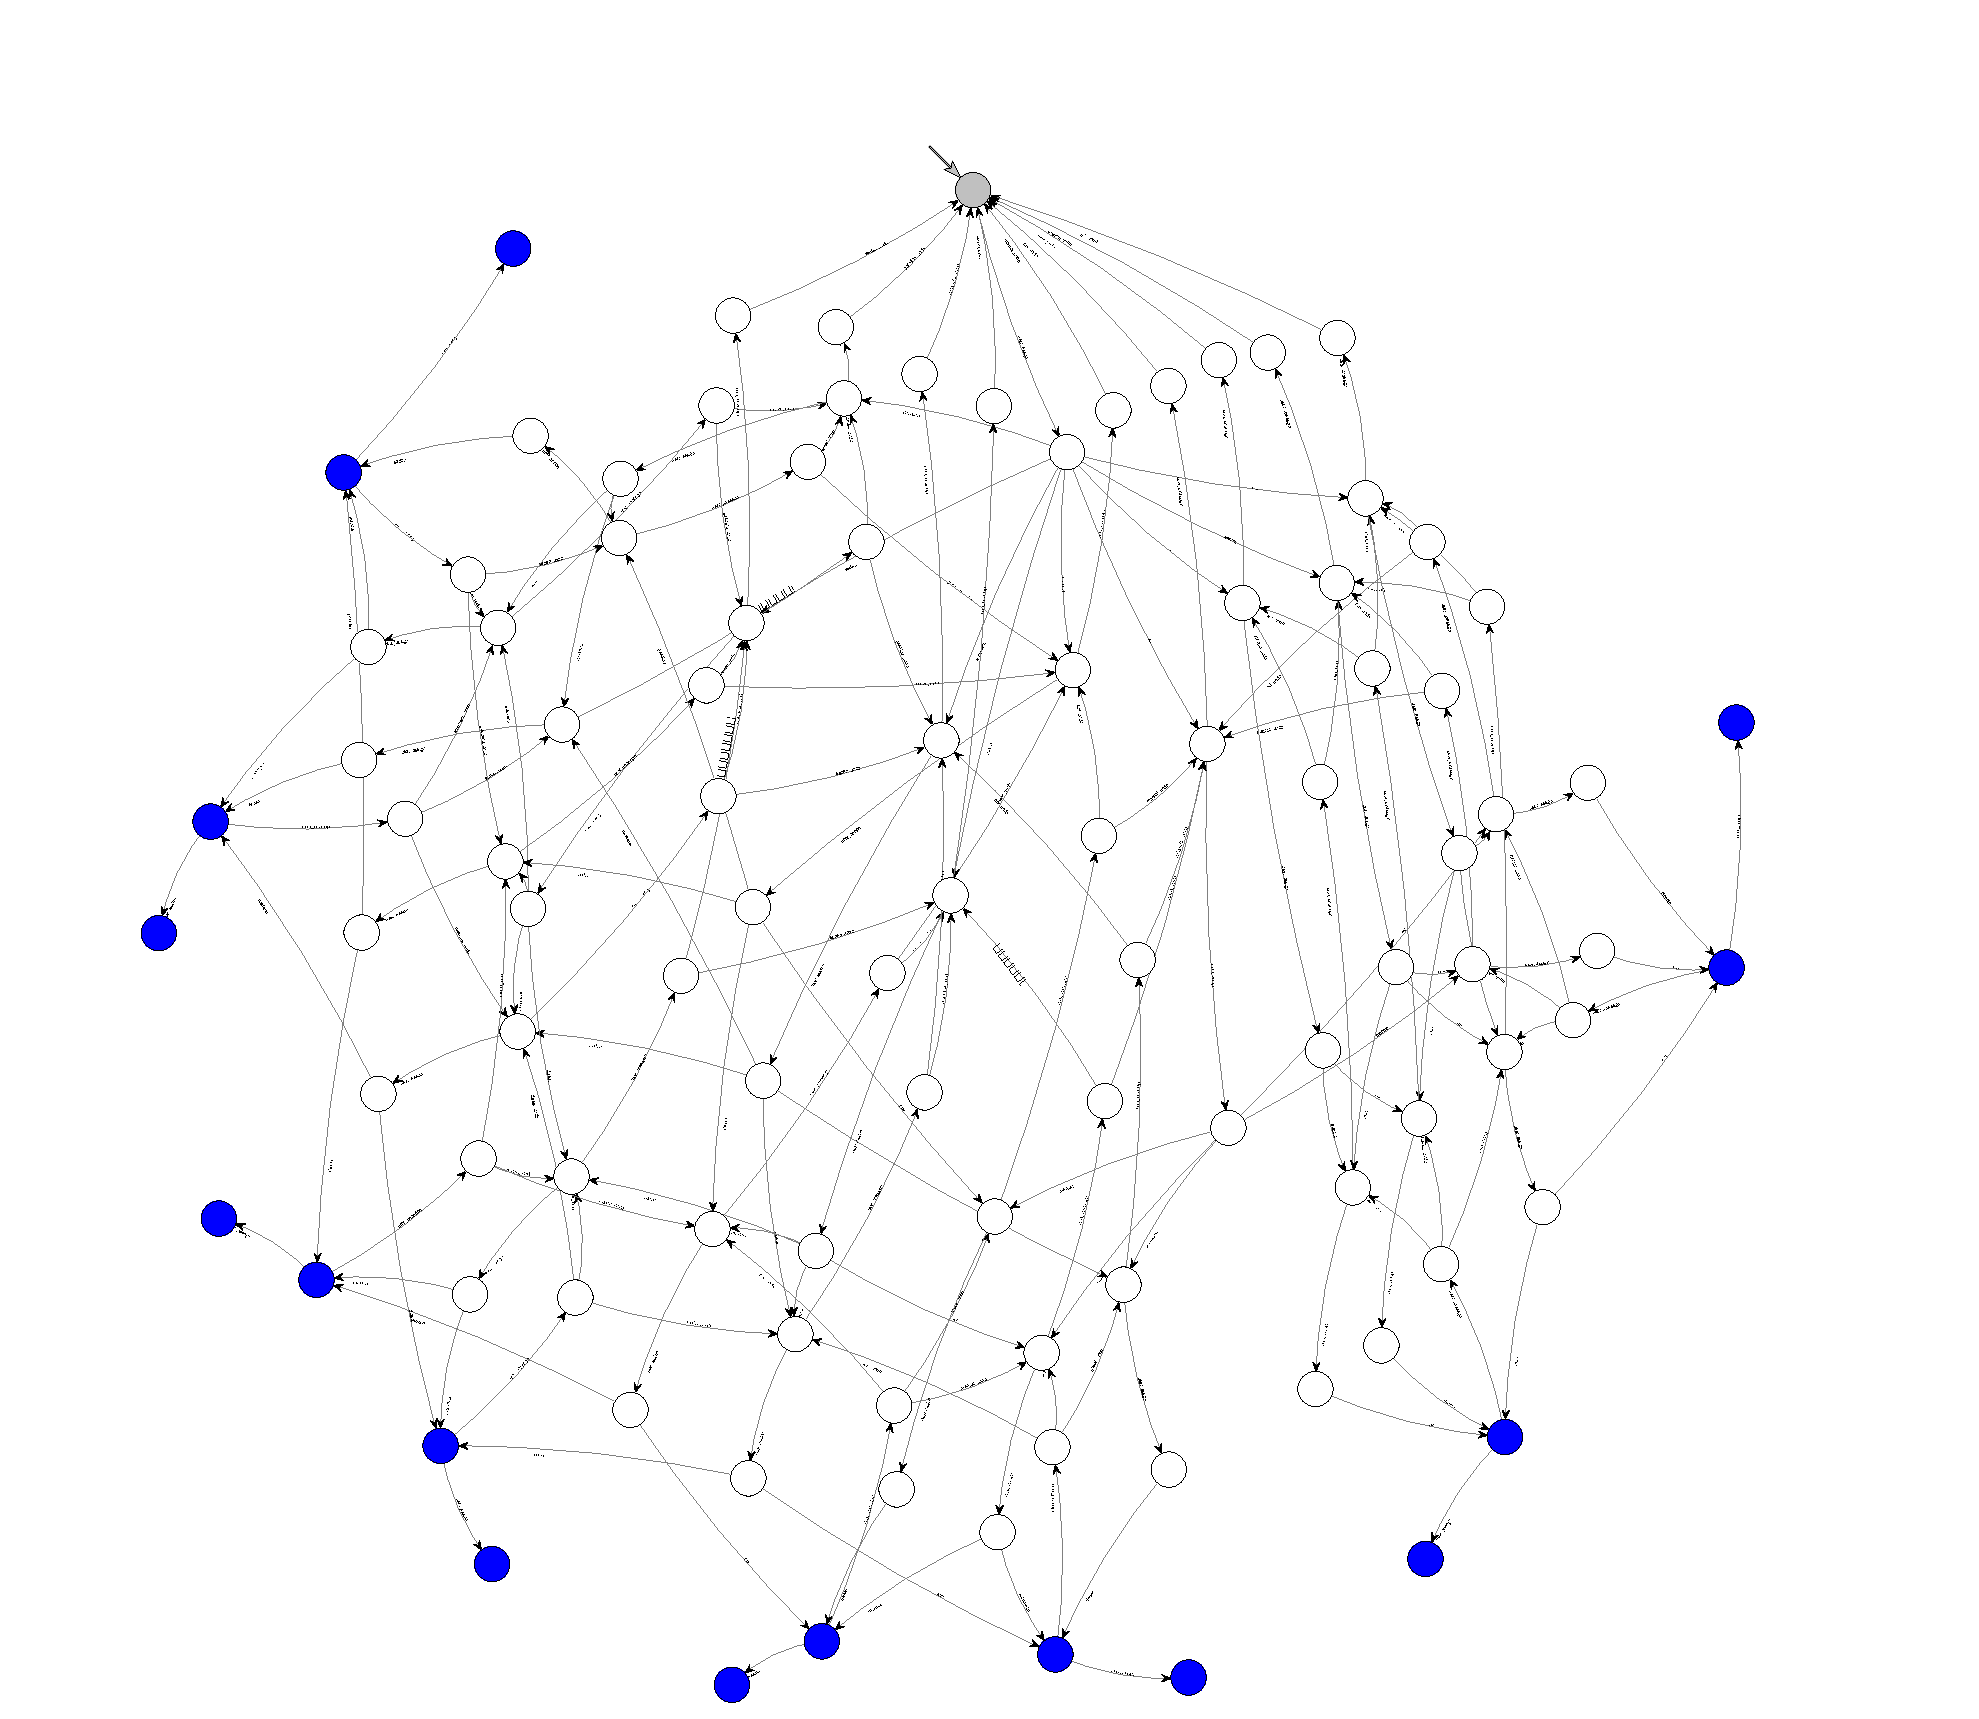
\includegraphics[width=0.8\textwidth]{kappa/images/supervisor}
\caption{An example of a supervisor.\label{fig:kappa-sup}}
\end{figure}

\lipsum[10-15]



%   .x~~"*Weu.
%  d8Nu.  9888c
%  88888  98888
%  "***"  9888%
%       ..@8*"
%    ````"8Weu
%   ..    ?8888L
% :@88N   '8888N
% *8888~  '8888F
% '*8"`   9888%
%   `~===*%"`
%
%%%%%%%%%%%%%%%%%%%%%%%%%%%%%%%
%%%%%%%%%%%%%%%%%%%%%%%%%%%%%%%
\chapter{Methods\label{ch:methods}}
%%%%%%%%%%%%%%%%%%%%%%%%%%%%%%%

\lipsum
